\documentclass[main.tex]{subfiles} % Subfile-Class


% ============================================================================== %
%                            Subfile document                                    %
% ============================================================================== %

\begin{document}

% Template

\subsubsection{Greifeinheit}


Die Abbildung~\ref{fig:Greifereinheit} veranschaulicht das Greiferkonzept des Roboters. Dieses Konzept wurde basierend auf der Evaluierung 
im Anhang~\ref{appendix:Greifereinheit} weiterentwickelt. Im folgenden Abschnitt wird die Funktionsweise des Greifers im Detail beschrieben.

\begin{figure}[H]
    \centering
    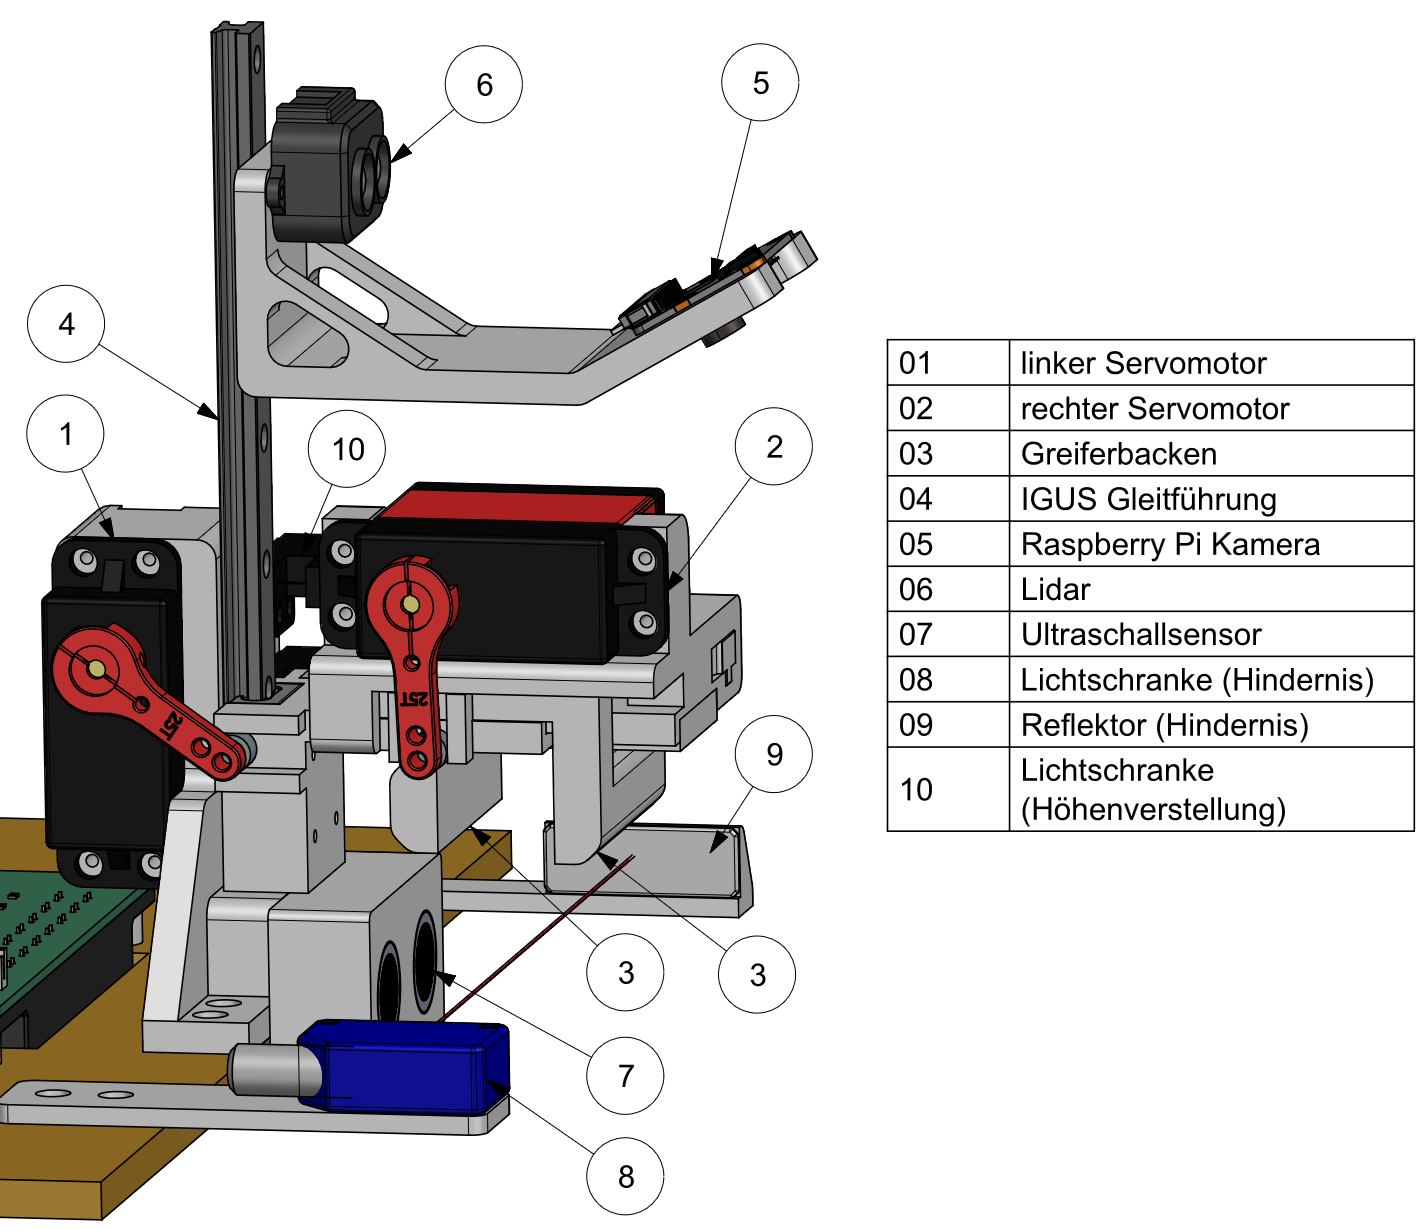
\includegraphics[width=0.75\textwidth]{Greifereinheit_Uebersicht.png}
    \caption{Greifereinheit}~\label{fig:Greifereinheit}
\end{figure}

Der Greifer verfügt über zwei Backen, die parallel zueinander verschoben werden, um das Hindernis sicher zu greifen. 
Dieser Vorgang wird von einem Servomotor gesteuert. Konkret bewegt der Hebel vom Servomotor eine der beiden Backen horizontal. 
Diese Backe ist mit einer Zahnstange ausgestattet, die ein innenliegendes Zahnrad antreibt. Das Zahnrad überträgt die 
Bewegung auf die gegenüberliegende Backe, sodass sich beide Backen synchron, aber in entgegengesetzter Richtung bewegen.
In der Abbildung~\ref{fig:Zahnrad und Zahnstange} ist dies dargestellt.

\begin{figure}[H]
    \centering
    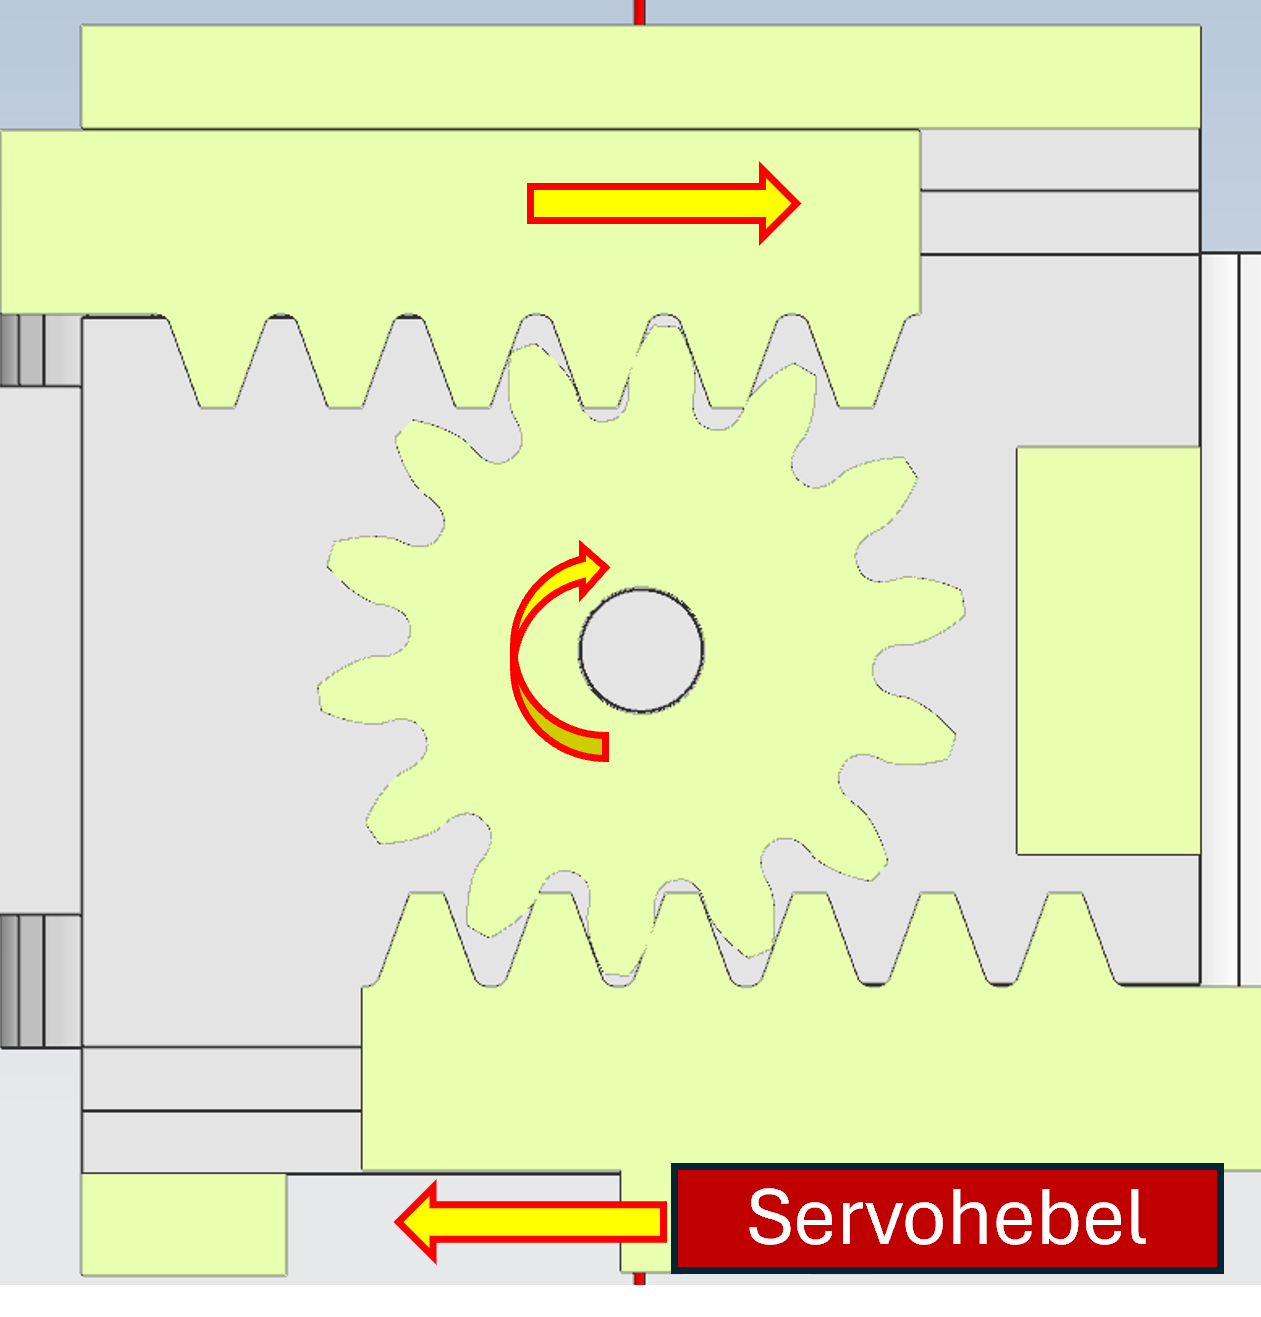
\includegraphics[width=0.5\textwidth]{Zahnrad_und_Zahnstange.png}
    \caption{Zahnrad und Zahnstange}~\label{fig:Zahnrad und Zahnstange}
\end{figure}


In Abbildung~\ref{fig:Hinderniss heben Ablauf} ist der Ablauf des Greifvorgangs schematisch dargestellt. Die einzelnen Schritte werden durch gelbe Pfeile visualisiert:

\paragraph{Positionierung der Greifeinheit} 
Von 1 zu 2 dreht der linke Servomotor die Greifeinheit entlang einer Gleitführung nach unten, wenn ein Hindernis erkannt wurde.

\paragraph{Greifen des Hindernisses} 

Von 2 zu 3 bewegt der rechte Servomotor die Backen horizontal, wodurch sich beide Backen parallel schliessen und das Hindernis fixieren.

\paragraph{Anheben des Hindernisses} 

Von 3 zu 4 dreht der linke Servomotr die Greifeinheit leicht nach oben, wodurch das Hindernis vom Boden abgehoben wird. 
Dies ermöglicht es, das Hindernis sicher zu transportieren.

\begin{figure}[H]
    \centering
    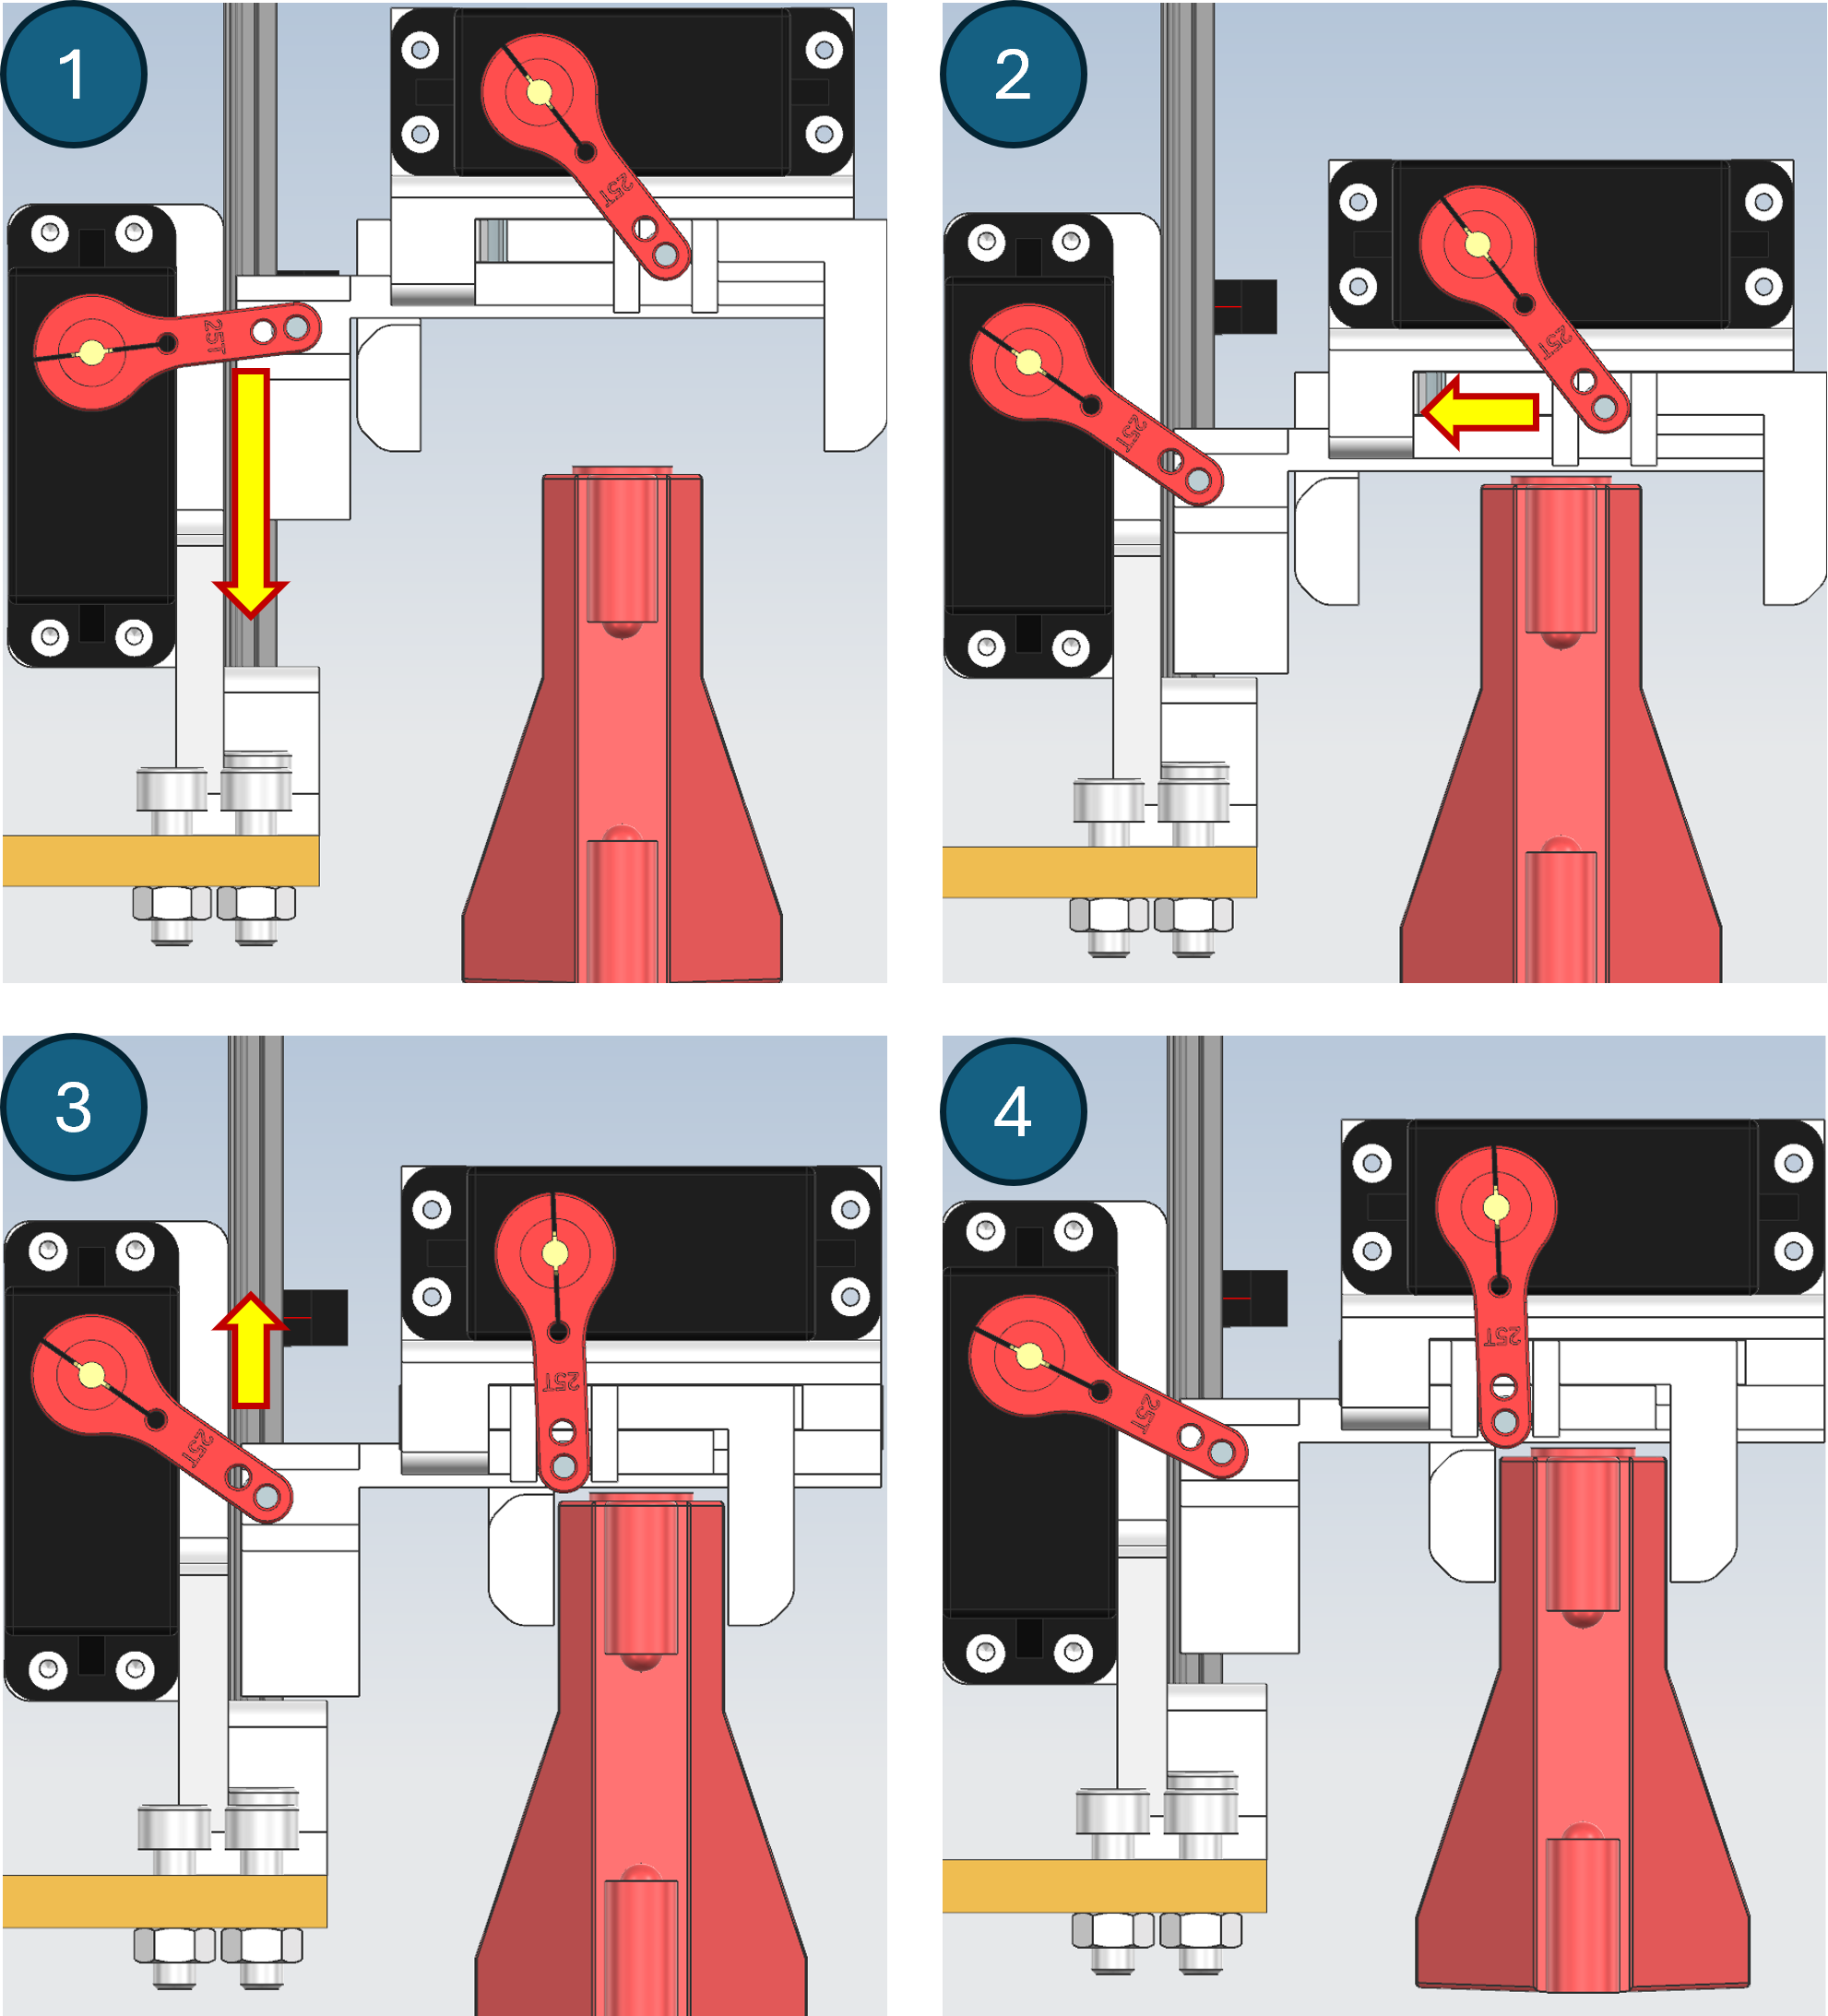
\includegraphics[width=1\textwidth]{Hinderniss_heben_Ablauf.png}
    \caption{Hinderniss heben Ablauf}~\label{fig:Hinderniss heben Ablauf}
\end{figure}


\subsubsection*{Sensorenplatzierung}

In diesem Abschnitt werden die verschiedenen Sensoren an der Greifereinheit beschrieben

\paragraph{Ultraschallsensor und Lidar}
Der Ultraschallsensor ist auf der Höhe XX positioniert um einen Hindernis zu erkennen 
und der Lidar ist auf der Höhe XX platziert um einen Pylon zu erkennen.
Die Details für diese Höhe wird im Kap. XX erklärt.


\paragraph{Lichtschranke Hindernis}
Diese Lichtschranke ist für die genauere Positionsbestimmung des Hindernis vorhanden.
Diese wurde auf der Höhe XX positioniert. Möglicherweise wird dieser nicht benötigt, falls der Ultraschallsensor 
genug zuverlässig funktioniert.

\paragraph{Raspberry Pi Kamera}
Die Raspberry Pi Kamera ist auf der Höhe XX montiert, sodass sie einen Radius von mindestens 150 mm abdeckt.
So kann sichergestellt werden, dass die maximalen 120 mm Knotenpunkte und die jeweiligen Abgänge detektiert werden können


\paragraph{Lichtschranke Endposition für Höhenverstellung}
Diese Lichtschranke ist für eine Rückmeldung für die oberen Endschlag des Höhenverstellung des Greifers vorgesehen.
Jedoch kann diese wie bei der unteren Endposition durch eine physische Blockade realisiert werden. Dies wird im PREN 2 getestet.







\end{document}
